% ======================================================================
%  UAM-TOPOMAT — Poster A0 moderne (841 x 1189 mm), 3 colonnes
%  Université Amadou Mahtar Mbow / UFR STA / Cellule Physique
%  Ndiogou Ndiaye — Année universitaire 2026 – 2027
%  Compilation : pdflatex poster.tex  (1 seule page A0)
% ======================================================================
\documentclass[a0paper,portrait]{article}

\usepackage[utf8]{inputenc}
\usepackage[T1]{fontenc}
\usepackage[french]{babel}
\usepackage{graphicx}
\usepackage{xcolor}
\usepackage[a0paper,portrait,left=14mm,right=14mm,top=12mm,bottom=12mm]{geometry}
\usepackage{tcolorbox}
\tcbuselibrary{skins}
\usepackage[hidelinks]{hyperref}

\pagestyle{empty}
\parindent   = 0pt
\parskip     = 0pt

\definecolor{glacier}{HTML}{F1F5F9}
\definecolor{navy}{HTML}{0F294A}
\definecolor{solar}{HTML}{F59E0B}
\definecolor{ink}{HTML}{152734}
\definecolor{muted}{HTML}{5B7183}
\definecolor{green}{HTML}{0B6E4F}
\definecolor{violet}{HTML}{7C3AED}
\definecolor{white}{HTML}{FFFFFF}
\definecolor{pastelA}{HTML}{F8FAFC}
\definecolor{pastelB}{HTML}{EFF6FF}
\definecolor{pastelC}{HTML}{ECFDF5}
\definecolor{emerald}{HTML}{047857}
\definecolor{gold}{HTML}{B45309}
\pagecolor{glacier}

\graphicspath{{../results/figures/}{./}}

\newlength{\kpiw}
\setlength{\kpiw}{\dimexpr(\textwidth-24mm)/4\relax}
\newlength{\colw}
\setlength{\colw}{\dimexpr(\textwidth-18mm)/3\relax}
\newlength{\colheight}
\setlength{\colheight}{700mm}

\newcommand{\sect}[1]{\textcolor{navy}{\fontsize{56}{64}\selectfont\textbf{#1}}\par\vspace{5mm}}
\newcommand{\bulletline}[1]{%
  \textcolor{green}{\fontsize{38}{38}\selectfont\textbf{\textbullet}}\quad
  \textcolor{ink}{\fontsize{38}{54}\selectfont #1}\par\vspace{5mm}}
\newcommand{\capfig}[1]{\textcolor{muted}{\fontsize{26}{31}\selectfont #1}\par}

\newcommand{\kpi}[4]{%
\begin{tcolorbox}[width=\kpiw,colback=#1,colframe=#1,boxrule=0pt,
                   arc=5mm,outer arc=5mm,
                   left=6mm,right=6mm,top=12mm,bottom=12mm,nobeforeafter]
  \color{#2}{\fontsize{104}{110}\selectfont\textbf{#3}}\par\vspace{3mm}
  \color{#2}{\fontsize{28}{33}\selectfont #4}
\end{tcolorbox}}

\newcommand{\champcard}[3]{%
\begin{tcolorbox}[width=\linewidth,colback=white,colframe=#1,boxrule=1.2mm,
                   arc=4mm,outer arc=4mm,
                   left=6mm,right=6mm,top=5mm,bottom=5mm,nobeforeafter]
   \textcolor{#1}{\fontsize{32}{38}\selectfont\textbf{#2}}\par\vspace{3mm}
   \textcolor{ink}{\fontsize{28}{38}\selectfont #3}
\end{tcolorbox}}

\tcbset{uamcard/.style={%
  enhanced,arc=6mm,outer arc=6mm,boxrule=0.9mm,
  left=5mm,right=5mm,top=4mm,bottom=4mm,
  toptitle=2.5mm,bottomtitle=2.5mm,
  coltitle=white,fonttitle=\fontsize{38}{44}\selectfont\bfseries,
  width=\linewidth,before skip=0pt,after skip=0pt}}

\newtcolorbox{cardnavy}[2][pastelB]{uamcard,colback=#1,colframe=navy,
  colbacktitle=navy,title={#2}}
\newtcolorbox{cardemerald}[2][pastelC]{uamcard,colback=#1,colframe=emerald,
  colbacktitle=emerald,title={#2}}
\newtcolorbox{cardgold}[2][pastelA]{uamcard,colback=#1,colframe=gold,
  colbacktitle=gold,title={#2}}

\begin{document}

% ----------------------------------------------------------------------
% BANDEAU SUPÉRIEUR BLEU MARINE + LISERÉ OR + LOGO + QR CODE
% ----------------------------------------------------------------------
\noindent\hspace*{-14mm}\begingroup\setlength{\fboxsep}{0pt}%
\colorbox{navy}{\parbox{\paperwidth}{%
  \vspace{9mm}%
  \begin{minipage}[c]{42mm}\hspace{5mm}
\includegraphics[width=36mm]{logo_uam.png}\end{minipage}\hfill
  \begin{minipage}[c]{660mm}
    \textcolor{white}{\fontsize{88}{94}\selectfont\textbf{UAM-TOPOMAT}}\\[3mm]
    \textcolor{solar}{\fontsize{36}{42}\selectfont\textbf{Matériaux quantiques \& stockage pour le climat sahélien}}\\[3mm]
    \textcolor{white!82!navy}{\fontsize{25}{30}\selectfont
      Université Amadou Mahtar Mbow $\cdot$ UFR Sciences et Technologies Avancées $\cdot$
      Cellule Physique $\cdot$ Ndiogou Ndiaye $\cdot$ 2026--2027}
  \end{minipage}\hfill
  \begin{minipage}[c]{92mm}\centering
    
\includegraphics[width=50mm]{qr_uam_topomat.png}\\[2mm]
    \textcolor{white}{\fontsize{23}{27}\selectfont\textbf{Démo interactive}}\\[1mm]
    \textcolor{solar}{\fontsize{23}{27}\selectfont\textbf{onrender.com}}
  \end{minipage}%
  \vspace{9mm}%
}}\endgroup\par
\vspace{3mm}
\noindent\hspace*{-14mm}{\color{solar}\hrule height 2.5mm width \paperwidth}\par
\vspace{9mm}

% ----------------------------------------------------------------------
% BANDEAU DE CARTES KPI (4 chiffres géants)
% ----------------------------------------------------------------------
\noindent
\kpi{green}{white}{+29,1\,\%}{Rendement Matam}\hfill
\kpi{navy}{white}{98,11\,\%}{Rétention MXène}\hfill
\kpi{solar}{navy}{42,60}{FCFA/kWh Matam}\hfill
\kpi{violet}{white}{28,56\,t}{CO$_2$ évitées/an}\par
\vspace{11mm}

% ----------------------------------------------------------------------
% TROIS COLONNES ÉQUILIBRÉES — 8 CARTES AUX COULEURS UAM
% ----------------------------------------------------------------------
\noindent
\begin{minipage}[t][\colheight][t]{\colw}
\raggedright

\begin{cardnavy}{1. Le défi sahélien}
\bulletline{1\,500--2\,200 kWh/m$^2$/an de soleil}
\bulletline{47\,$^\circ$C à Matam : le rendement chute}
\bulletline{Twin Transition : énergie + numérique souverain}
\end{cardnavy}

\vfill
\begin{cardemerald}{2. Pipeline en 5 étapes}
\bulletline{Cristallographie + Tight-Binding}
\bulletline{Berry / Chern : topologie certifiée}
\bulletline{Optique AM1.5G + climat sahélien}
\bulletline{Transport $J(V)$ + stockage MXène}
\bulletline{Découverte inverse NSGA-II}

\begin{center}
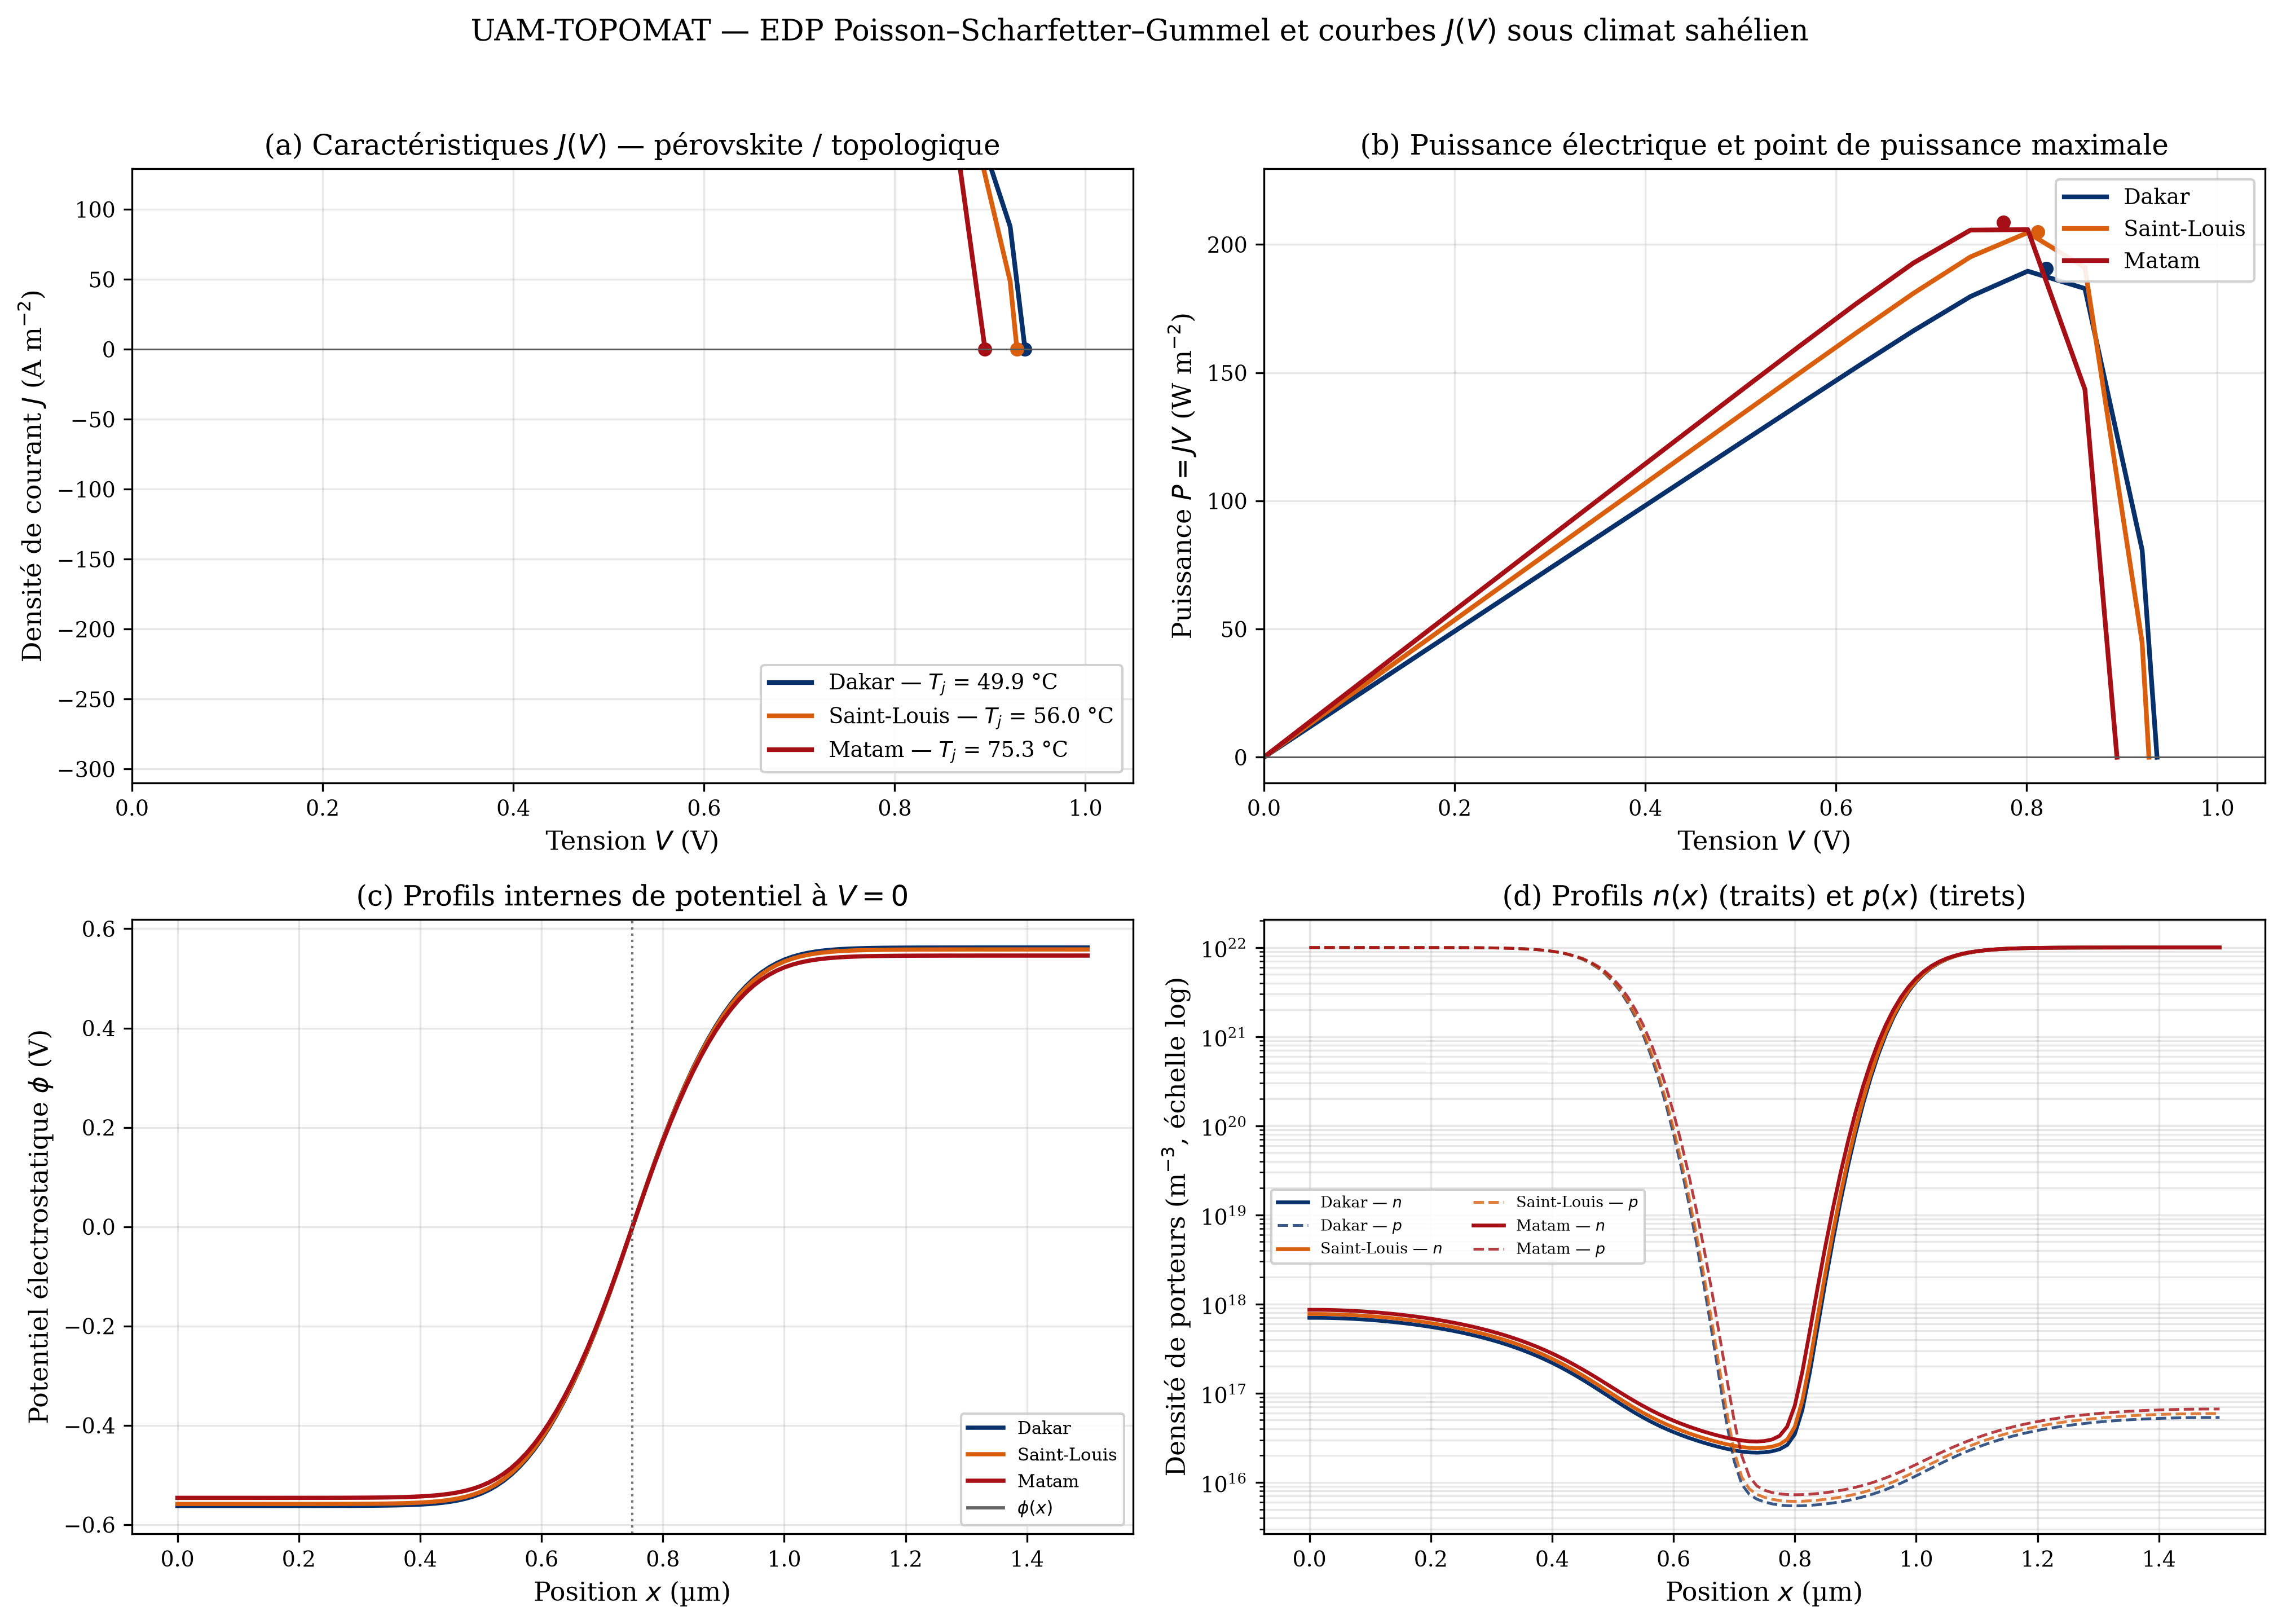
\includegraphics[width=\linewidth]{night6_jv_curves_sahel.png}\\[2mm]
\capfig{Courbes $J(V)$ en conditions sahéliennes --- 300 dpi}
\end{center}
\end{cardemerald}

\vfill
\begin{cardgold}{3. Zéro dépendance SciPy}
\bulletline{6 théorèmes certifiés symboliquement}
\bulletline{36 bornes physiques vérifiées}
\bulletline{316 tests automatisés}
\end{cardgold}

\end{minipage}\hfill
\begin{minipage}[t][\colheight][t]{\colw}
\raggedright

\begin{cardnavy}{4. 2\,000 matériaux criblés}
\bulletline{900 ABX$_3$ + 550 doubles + 550 MXènes}
\bulletline{Sans Pb ni Co, neutralité électrique}
\bulletline{Front NSGA-II : 198 solutions}

\begin{center}
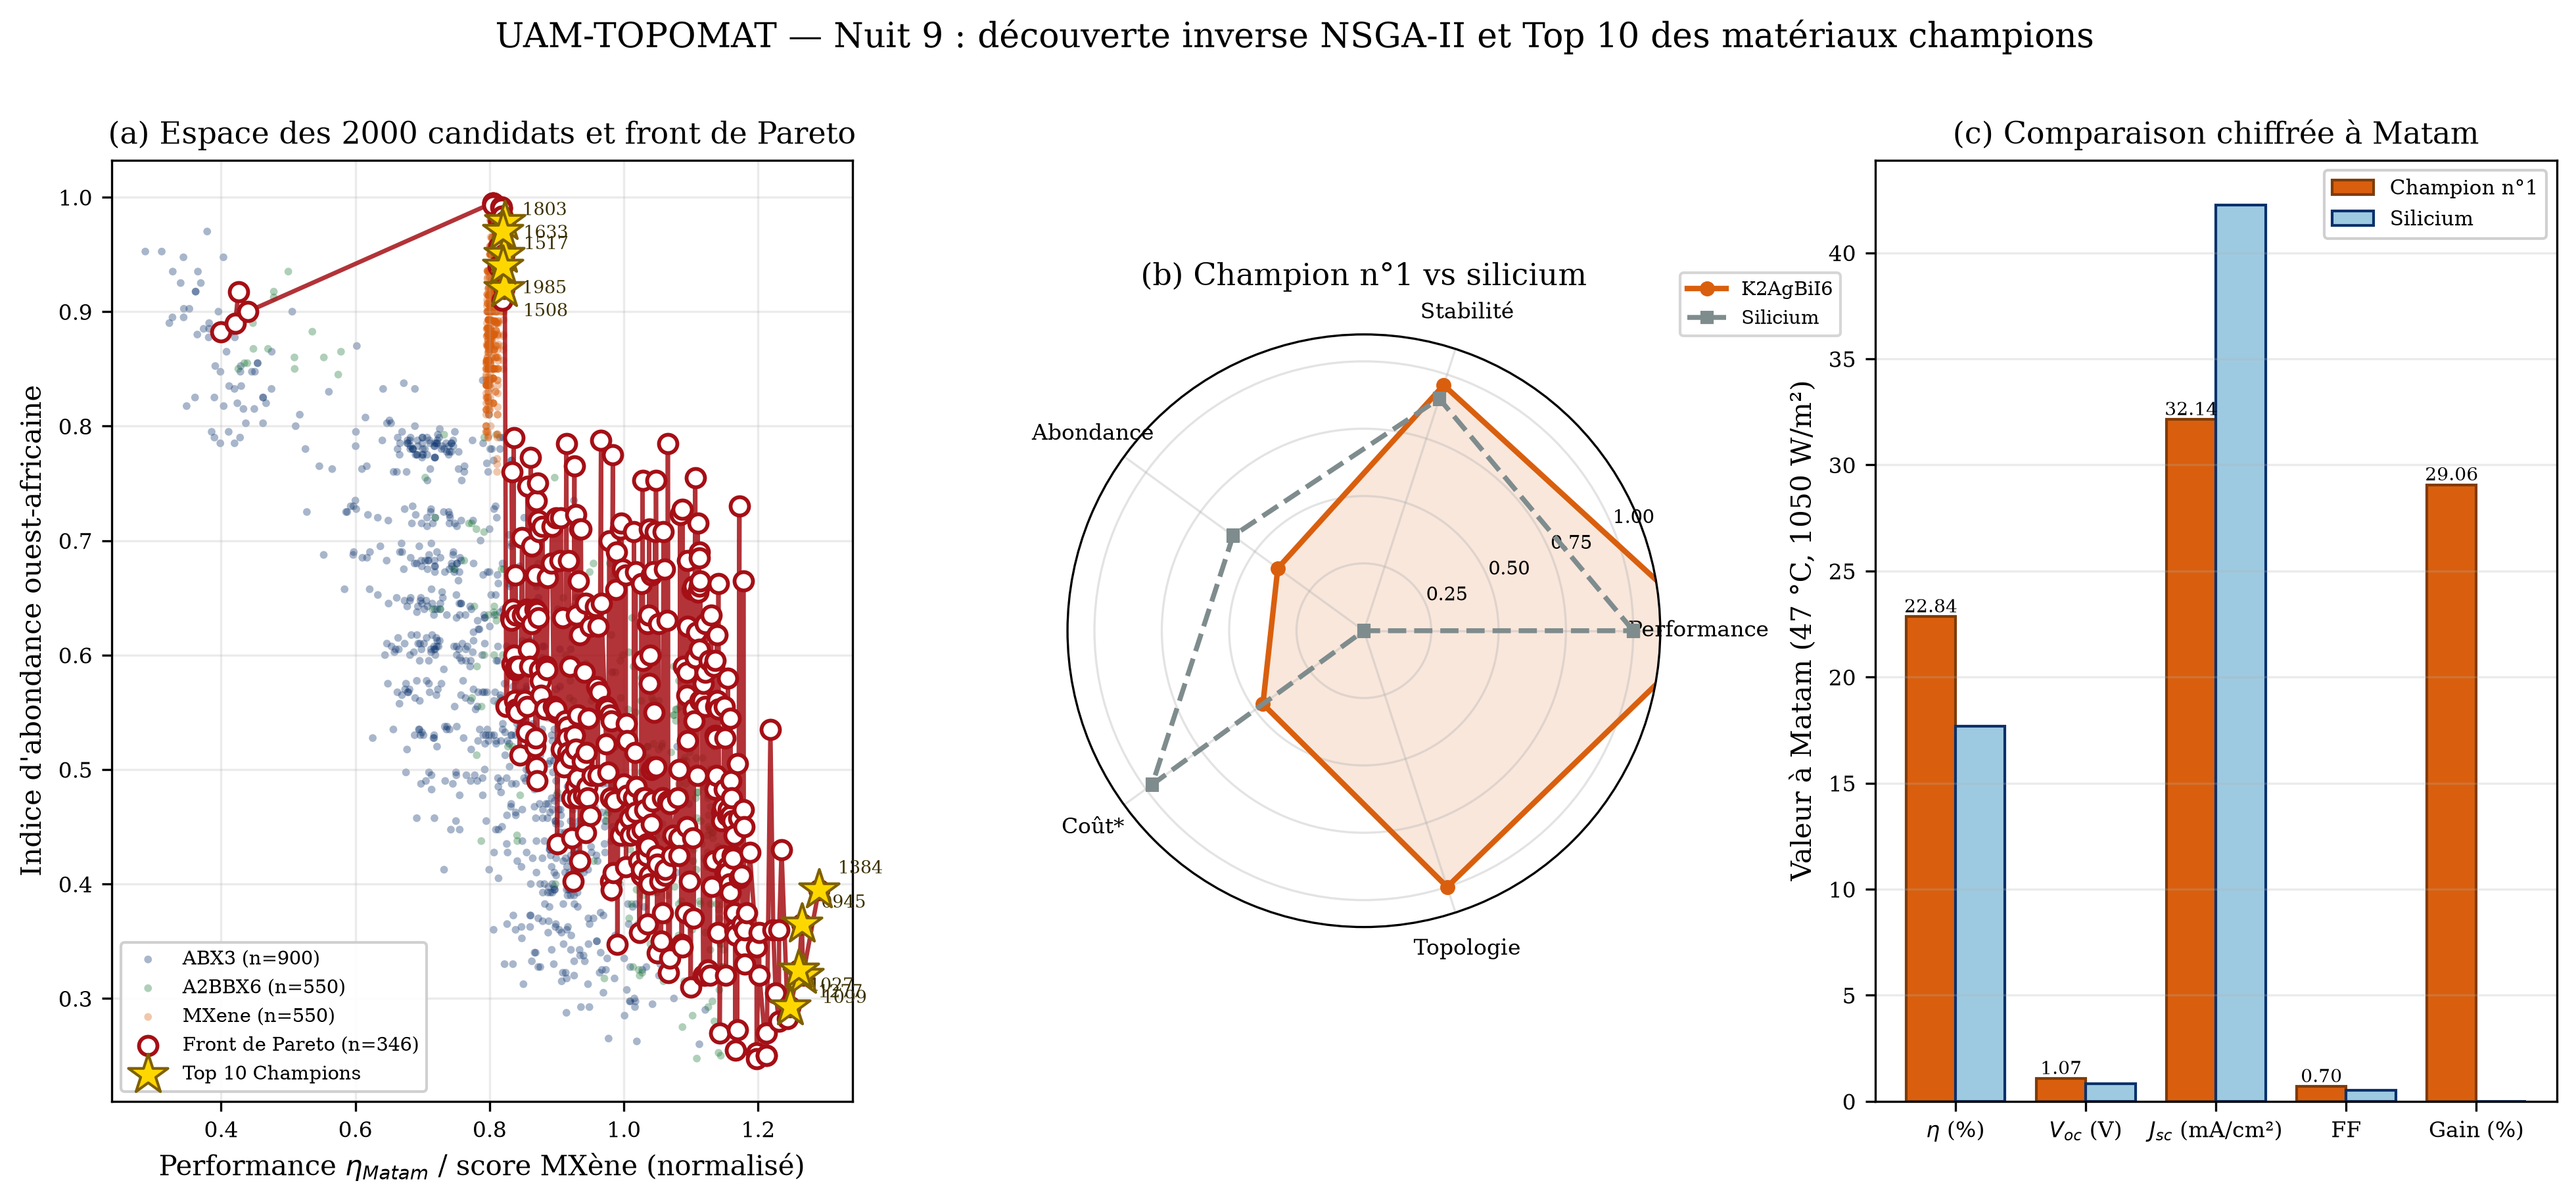
\includegraphics[width=\linewidth]{night9_pareto_discovery.png}\\[2mm]
\capfig{Espace de Pareto, front NSGA-II et Top 10 --- 300 dpi}
\end{center}
\end{cardnavy}

\vfill
\begin{cardemerald}{5. Les deux champions}

\champcard{green}{UAM-1384 --- K$_2$AgBiI$_6$ (solaire)}
  {Gap 1,390 eV $\cdot$ $C=+1$ $\cdot$ $\eta=22{,}84\,\%$ à 47\,$^\circ$C}
\vspace{6mm}
\champcard{violet}{UAM-1517 --- Ti$_3$C$_2$O$_2$ (stockage)}
  {Gap 1,865 eV $\cdot$ $C=-1$ $\cdot$ 5,97 Wh/kg à 47\,$^\circ$C}
\begin{center}
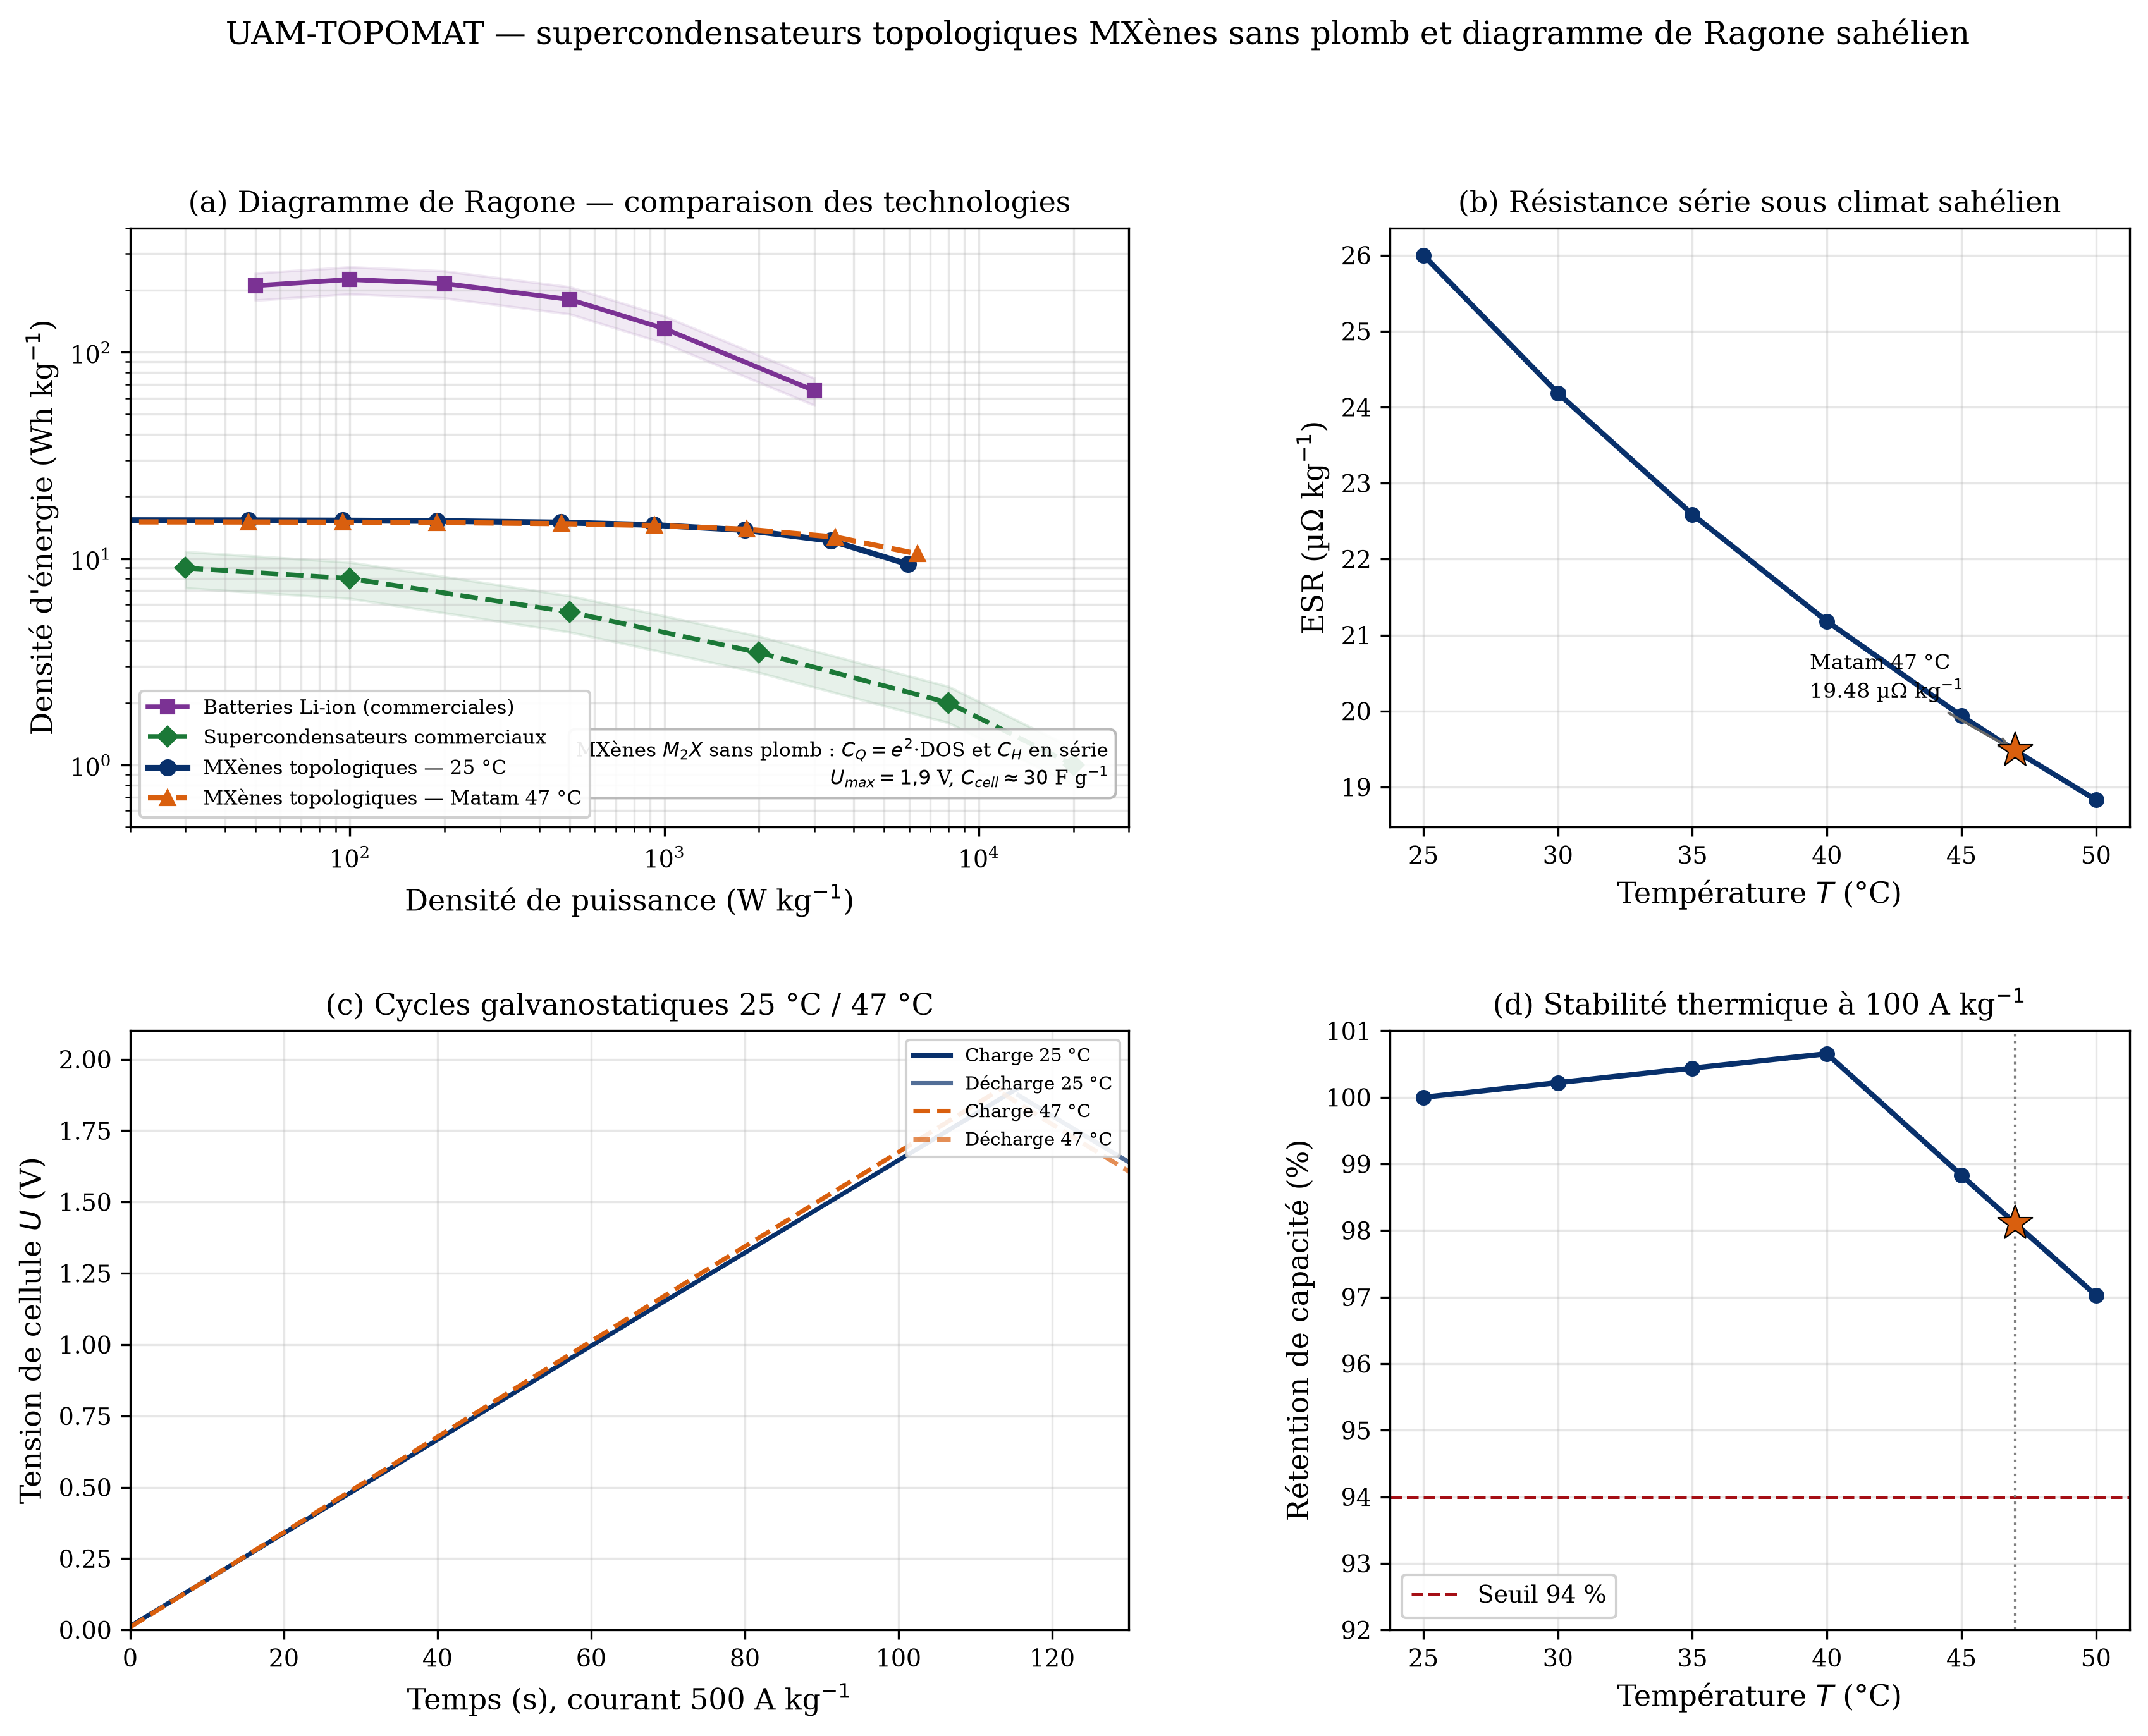
\includegraphics[width=\linewidth]{night7_ragone_mxene_sahel.png}\\[2mm]
\capfig{Ragone du supercondensateur MXène --- 300 dpi}
\end{center}
\end{cardemerald}

\end{minipage}\hfill
\begin{minipage}[t][\colheight][t]{\colw}
\raggedright

\begin{cardgold}{6. Impact au Sénégal}
\bulletline{Mini-centrale 100 kWc + 100 kWh}
\bulletline{Dakar $\cdot$ Saint-Louis $\cdot$ Matam}
\bulletline{220 FCFA/kWh $\cdot$ 0,55 t CO$_2$/MWh}

\begin{center}
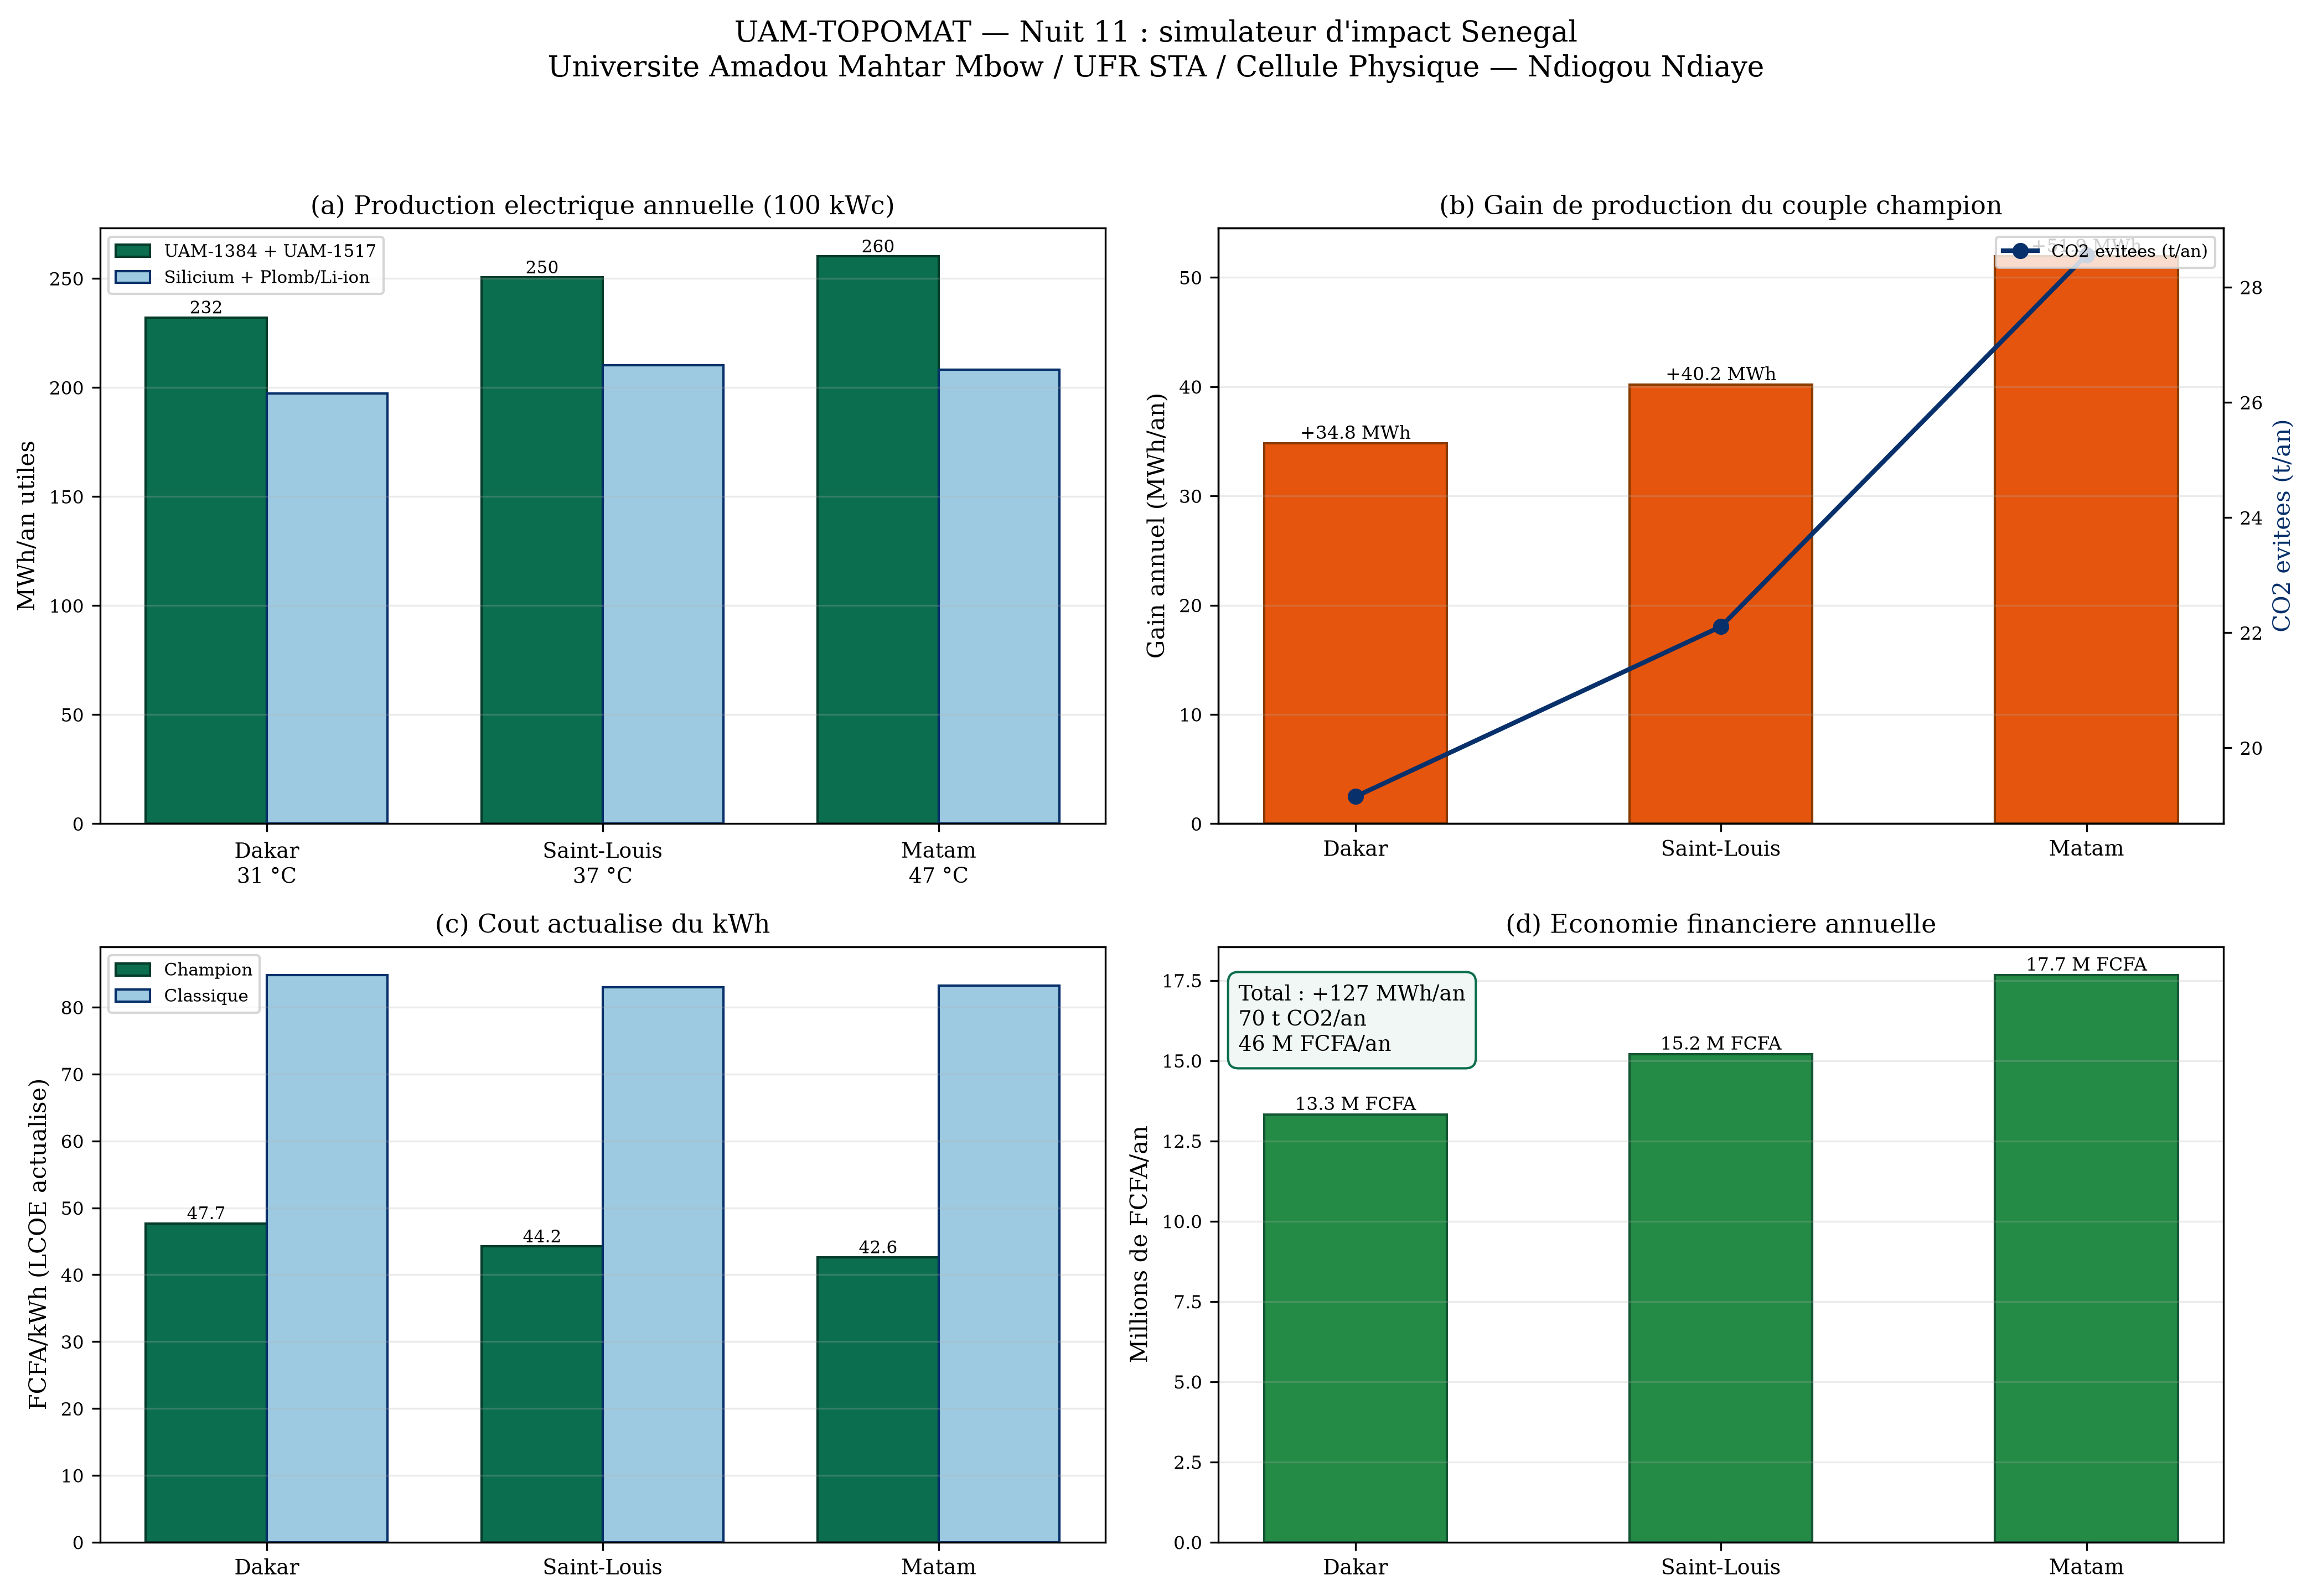
\includegraphics[width=\linewidth]{night11_senegal_impact.png}\\[2mm]
\capfig{Bilan multi-régions : MWh, CO$_2$, LCOE et FCFA --- 300 dpi}
\end{center}
\vspace{5mm}

\textcolor{navy}{\fontsize{28}{35}\selectfont\textbf{+126,9 MWh/an $\cdot$ 69,8 t CO$_2$/an $\cdot$ 46,2 M FCFA/an $\cdot$ baisse LCOE 44--49\,\%}}
\end{cardgold}

\vfill
\begin{cardnavy}{7. Démonstration live}
\bulletline{Serveur FastAPI 100\,\% hors ligne}
\bulletline{Matériau, ville et température au choix}
\bulletline{Pipeline complet en un seul clic}
\bulletline{Lancer : \texttt{LANCER\_DEMO\_JURY.bat}}
\end{cardnavy}

\vfill
\begin{cardemerald}{8. Perspectives}
\bulletline{DFT + couplage spin--orbite}
\bulletline{Synthèse de K$_2$AgBiI$_6$ et Ti$_3$C$_2$O$_2$}
\bulletline{Prototype 1 kWc à Matam}
\end{cardemerald}

\vfill
{\color{solar}\hrule height 1.2mm}\par\vspace{4mm}
\textcolor{navy}{\fontsize{25}{30}\selectfont\textbf{UAM / UFR STA / Cellule Physique --- Ndiogou Ndiaye --- 2026--2027}}

\end{minipage}

\end{document}
